\documentclass{article}

\usepackage[utf8]{inputenc}

% Language
\usepackage[french]{babel} %english

% Geometry
\usepackage[includehead, includefoot, margin=1.5cm]{geometry}
\usepackage{multicol}

% FLoat
\usepackage{float}

% Date format
\usepackage[yyyymmdd]{datetime}

% Hyperref
\usepackage[pdfborder={0 0 0}]{hyperref}

% Header and footer
\usepackage{fancyhdr}
\usepackage{lastpage}

% Fonts
%\usepackage{DejaVuSans}
%\usepackage{DejaVuSansMono}
%\usepackage{arev}
\usepackage{amsfonts}
\usepackage{amsmath}
\usepackage{amssymb}

% Colors
\usepackage[table]{xcolor}

% Illustrations
\usepackage{pdfpages}
\usepackage{graphicx}
\usepackage{wrapfig}
\usepackage{graphbox}
\usepackage{tikz}
\usepackage[fixed]{fontawesome5}

% Code listings
\usepackage[breakable]{tcolorbox}
\usepackage{listings}

% Tables% Captions
\usepackage{tabularx}
\usepackage{arydshln}
\usepackage{multirow}

% Lists
\usepackage{enumitem}

% Bibliography
\usepackage{csquotes}
\usepackage[backend=biber, style=numeric, sorting=none]{biblatex}

% Glossaries
\usepackage[acronym]{glossaries}
%, toc, nogroupskip, numberedsection, nonumberlist, section=section

% Captions
\usepackage[hypcap=false]{caption}

% Text
\usepackage{mfirstuc}
\usepackage[squaren,Gray]{SIunits}

% Math
\usepackage{tensor}
% Date format
\renewcommand{\dateseparator}{--}

% Header and footer
\pagestyle{fancy}
\fancyfoot[L]{\today}
\fancyfoot[C]{}
\fancyfoot[R]{Page \thepage \ of \pageref*{LastPage}}

% Fonts
\renewcommand{\familydefault}{\sfdefault}

% Colors
\definecolor{Blue}{RGB}{031, 119, 180}
\definecolor{Orange}{RGB}{255, 127, 14}
\definecolor{Green}{RGB}{044, 160, 44}
\definecolor{Red}{RGB}{214, 039, 040}
\definecolor{Grey}{RGB}{176, 176, 176}
\definecolor{Mines}{RGB}{079, 054, 154}

% Code listings
\tcbset{colback=white, coltext=black, colframe=Mines, boxrule=0.06cm}
\lstset{basicstyle=\normalsize\ttfamily,
        keywordstyle=\color{Orange},
        stringstyle=\color{Green},
        identifierstyle=\color{black},
        commentstyle=\color{Grey},
        showstringspaces=false}

% Lists
%\setlength{\parindent}{0pt}
%\setlist[itemize]{leftmargin=*}
\setitemize[1]{label=\( \bullet \)}
\setitemize[0]{label=\( \circ \)}

% Bibliography
\addbibresource{input/references.bib}

% Glossaries
\makeglossaries
%\makenoidxglossaries

% Maths
\everymath{\displaystyle}

%no need to be alphabetically sorted

\newglossaryentry{pacman}
{
  name={Pac-Man},
  description={Jeu qui consiste à déplacer Pac-Man, un personnage à l'intérieur d'un labyrinthe, afin de lui faire manger toutes les pac-gommes qui s'y trouvent en évitant d’être touché par des fantômes.}
}

\newglossaryentry{fruit}
{
	name={fruit},
	description={L'objectif du jeu},
	first={pac-gomme}
}



%mechanical study
\newcommand{\x}[1] {\vec{x_#1}}
\newcommand{\y}[1] {\vec{y_#1}}
\newcommand{\z}[1] {\vec{z_#1}}
\newcommand{\base}[1] {
  (\x#1,\y#1,\z#1)
}
\newcommand{\torseur}[2] {%\torseur{force}{solide}
  \left\{
  T_{#1\to #2}
  \right\}
}
\newcommand{\Torseur}[4] {%\Torseur{point}{R}{M}{base}
  \tensor[_{#1}]{
  \left\{
  \begin{array}{l}
    #2 \\
    #3
  \end{array}
  \right\}
  }{_{#4}}
}



\newcommand{\PCGridContour}{ %Contour grille
	\fill[black, very thick] (0,0) rectangle (8,6);
}

\newcommand{\PCGridInside}{ %Grille
	\foreach \i in {1,...,7} {
		\draw [very thin,gray,dotted] (\i,0) -- (\i,6);
	}
	
	\foreach \i in {1,...,5} {
		\draw [very thin,gray,dotted] (0,\i) -- (8,\i);
	}
}

\newcommand{\PCGridContourNum}{ %Contour grille numéroté
	\foreach \i in {0,...,7} {
		\draw (\i+0.5,6) node[above]{$\i$};
	}
	\foreach \i in {0,...,5} {
		\draw (0,5.5-\i) node[left]{$\i$};
	}
}

\newcommand{\PCGridInsideNum}{ %Intérieur grille numéroté
	\foreach \i in {0,...,7} {
		\foreach \j in {0,...,5} {
			\draw (\i+0.5,5.5-\j) node[white]{$(\i,\j)$};
		}
	}
}

\newcommand{\PCGridAxis}{ %Axes
	\fill[rounded corners, color=cyan!20] (8.5,3.7) rectangle (11.5,5.4);
	\draw (10,5.4) node[above] {Axes};
	
	\fill[color=black] (9.5,5) circle [radius=2pt];
	\draw[->] (9.5,5) -- ++(0,-1) node[right] {$\vec{y}$};
	\draw[->] (9.5,5) -- ++(1,0) node[below] {$\vec{x}$};
}

\newcommand{\PCGridDirection}{ %Direction
	\fill[rounded corners, color=cyan!20] (8.5,1) rectangle (11.5,3);
	\draw (10,3) node[above] {Directions};
	\fill[color=black] (10,2) circle [radius=2pt];
	\draw[->] (10,2) -- ++(0.5,0) node[right] {$up$};
	\draw[->] (10,2) -- ++(-0.5,0) node[left] {$down$};
	\draw[->] (10,2) -- ++(0,0.5) node[above] {$left$};
	\draw[->] (10,2) -- ++(0,-0.5) node[below] {$right$};
}

\newcommand{\PCGridFill}[3]{ %Colorie une case
	\fill[color=#3,opacity=0.4] (#1,5-#2) rectangle ++(1,1);
}

\newcommand{\PCGridWall}[2]{ %Construit un mur
	\draw[rounded corners, thick, color=blue] (#1+0.05,5.05-#2) rectangle ++(0.9,0.9);
	\fill[rounded corners, color=blue] (#1+0.1,5.1-#2) rectangle ++(0.8,0.8);
}

\newcommand{\PCPacMan}[3]{ %PacMan
	\fill[color=yellow!90!black, rotate around={#3:(#1+0.5,5.5-#2)}] (#1+0.5,5.5-#2) -- ++(0.283,0.283) arc (45:315:0.4) -- cycle ;	
}

%\newcommand{\PCFruit}[3]{ %Fruit
%	\fill[color=#3] (#1+0.5,5.5-#2) circle [radius=0.2];	
%}

\newcommand{\PCFruit}[3]{
	\foreach \rot in {0,...,5} {
		\fill[color=#3, rotate around={\rot*60:(#1+0.5,5.5-#2)}] (#1+0.68,5.5-#2) circle [radius=0.18];
	}
}

\newcommand{\PCGridUn}{
	\PCGridWall{0}{3}
	\PCGridWall{0}{4}
	\PCGridWall{1}{0}
	\PCGridWall{1}{1}
	\PCGridWall{2}{1}
	\PCGridWall{2}{3}
	\PCGridWall{2}{4}
	\PCGridWall{3}{1}
	\PCGridWall{3}{3}
	\PCGridWall{4}{5}
	\PCGridWall{5}{0}
	\PCGridWall{5}{5}
	\PCGridWall{6}{0}
	\PCGridWall{6}{2}
	\PCGridWall{7}{0}
	\PCGridWall{7}{2}
	\PCGridWall{7}{3}
	\PCGridWall{7}{4}
	\PCGridWall{7}{5}
	\PCFruit{5}{2}{red}
}



\begin{document}

\begin{titlepage}
	\begin{center}
		
		\textsc{\LARGE École des Mines de Saint Étienne}\\[2cm]
		
		\textsc{\Large Défi : Intelligence Artificielle}\\[1cm]
		\textsc{\Large UP3 - AI Practice and Technos: Simulation}\\[2cm]
		
		% Title
		{ \huge \bfseries Compte rendu du projet de simulation}
		\\[1cm]
		
\includegraphics[width=0.4\textwidth]{image/logo_mines.png}
		\\[2cm]
		
		% Author and supervisor
		\begin{minipage}{0.8\textwidth}
			\begin{flushleft} \large
				Kalomé \textsc{Botowamungu}\\[0.2cm]
				Nicolas \textsc{Dunou}\\[0.2cm]
				Étienne-Théodore \textsc{Prin}\\[0.2cm]
				Benjamin \textsc{Teyssier}\\[0.2cm]
				Timothé \textsc{Tournier}\\
			\end{flushleft}
		\end{minipage}
		
		\vfill
		
	\end{center}
\end{titlepage}


\tableofcontents \label{contents}

%\newpage

\section{Situation et solution proposée}
\subsection{Situations}
Nous avons adapté le jeu \Gls{pacman} pour la simulation multi-agents d'un système complexe. Les agents sont les \Glspl{pacman} qui ont pour objectif de récupérer les \glspl{fruit}, appelés \glspl{fruit} par la suite à travers le labyrinthe. Un exemple est la figure \ref{fig:exemple1}\\
\begin{figure}[!h]
	\begin{tikzpicture}[scale=1.6]
		\PCGridContour
		\PCGridInside
		\PCGridUn
		\PCPacMan{3}{2}{0}
		\PCGridLegend
	\end{tikzpicture}
	\caption{Exemple du jeu}
	\label{fig:exemple1}
\end{figure}

\section{Évaluation de notre solution}
Pour évaluer la performance de nos robots, le paramètre qui semble le plus pertinent est le nombre de pas de temps nécessaires pour que tous les fruits soient mangés par les pacmans.
Ainsi, deux études sont possibles:
-l’influence de la taille du plateau sur le temps nécessaire aux pacmans pour manger tous les fruits
-l’influence du nombre de pacmans sur le temps nécessaire aux pacmans pour manger tous les fruits
Comme le nombre de fruit est égal au nombre de pacman, le résultat n'est pas complètement analysable car la carte place les objectifs et les pacmans de façon pseudo-aléatoire. Cependant on peut noter que toute solution diminuant le nombre de pas en comparaison au cas où les pacmans n'ont aucune notion de répartition des objectifs est une amélioration du système. Notre indicateur de performance du système pour chaque situation est donc le nombre de pas nécessaires. Si nous souhaitons implémenter de nouvelles méthodes de répartition où de choix des trajectoires, il faudra juger leur performance en fonction de la moyenne du nombre de pas nécessaire dans les différentes configurations de l'environnement (nombre de pac-mans, taille de la carte). L'implémentation de ces différents algorithmes nous ayant déjà demandé un temps de travail très important nous n'avons pas pu réaliser la version basique de choix au hasard ou du choix le plus proche. Cependant, la solution que nous implémentons est obligatoirement plus efficace en terme de nombre de coups puisqu'elle teste toutes les répartitions dont celle qui ressortiraient des méthodes de choix précédentes.



\section{Résultat}

Dans la première étude, on fait varier le nombre de colonnes du plateau en conservant un nombre constant de lignes (20) et de \glspl{pacman} (2). Pour chaque taille de plateau donnée, on récupère le nombre de pas de temps pour 6 \textit{seeds} différents afin de faire une moyenne. On remarque qu’en augmentant, la taille du plateau a tendance à faire augmenter le temps nécessaire aux \glspl{pacman} pour manger tous les \glspl{fruit}.\\
Cela pouvait être plutôt prévisible car en augmentant la taille du plateau les \glspl{fruit} ont de fortes chances de se retrouver plus loin des \glspl{pacman} à l’initialisation.
En augmentant le nombre de tests avec des \textit{seeds} différents et des tailles encore plus grandes on aurait pu avoir une courbe de tendance plus précise qui pourrait peut-être nous donner la relation entre la taille du plateau et le temps de résolution.

\begin{figure}[H]
	\centering
	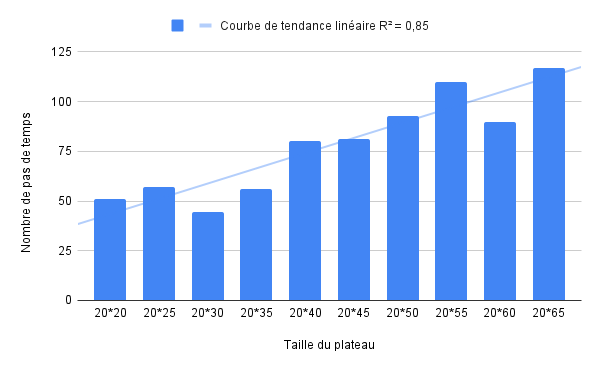
\includegraphics[width=0.8\textwidth]{image/resultat1}
	\caption{Nombre de pas de temps en fonction de la taille du plateau}
\end{figure}

Pour la seconde étude, on fait varier le nombre de \glspl{pacman} en conservant une taille constante pour le plateau, 20*20. Cette taille a été choisie car elle permet de ne pas avoir un temps de calcul trop long au-delà de 4 robots. 5 plateaux différents ont été testés en faisant varier le nombre de \glspl{pacman}. On ne peut pas voir directement de lien entre le temps mis par les \glspl{pacman} pour manger tous les \glspl{fruit} et le nombre de \glspl{pacman}.\\
Cela est certainement dû au fait que le nombre de \glspl{fruit} est le même que le nombre de \glspl{pacman} et qu'ils ne sont pas placés de façon aléatoire, donc leur nombre augmentent en même temps dans les tests. Ici aussi, des tests avec un plus grand nombre de plateaux et avec des nombres de \glspl{pacman} plus grands auraient potentiellement pû permettre d’établir un lien entre les deux données mises en jeu. Une amélioration de notre système pourrait être dans le futur de décorrelé le nombre d'objectifs et le nombre d'agents
\begin{figure}[H]
	\centering
	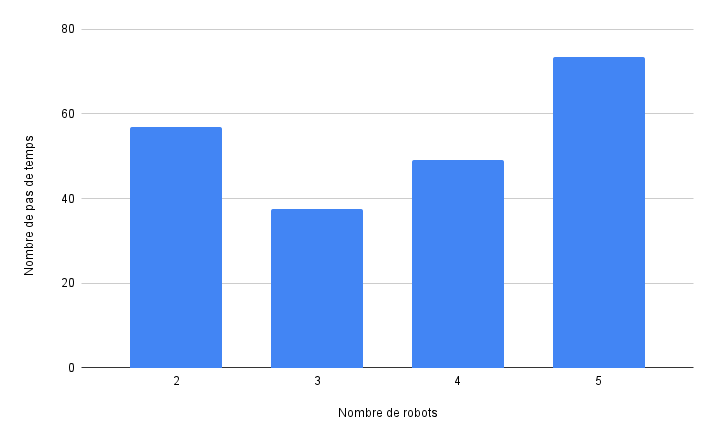
\includegraphics[width=0.8\textwidth]{image/resultat2}
	\caption{Nombre de pas de temps en fonction du nombre de robots}
\end{figure}


\section{Choix d'implémentation}

\subsection{Obtention d'itinéraire}
Pour que nos robots trouvent un chemin pour accéder à leurs objectifs de manière efficace, nous avons implémenté un algorithme de \textit{pathfinding}.

Comme expliqué plus haut, chaque robot n'a qu'une connaissance partielle de son environnement: il actualise une carte à mesure de ses déplacements. C'est à partir de cette carte que nous établissons un chemin vers l'objectif. 

Le robot calcule son itinéraire à l'aide d'un algorithme $A^\star$. Les positions sur la grilles munies de l'itinéraire pour y parvenir constituent les états du système considéré. 
Pour un état donné, l’ensemble des états atteignables considérés est l’ensemble des cases voisines inoccupées ou inconnues privé de la « case père ». La case père représente la case précédente, nous l’excluons pour que le robot ne considère pas de chemin incluant un retour sur ses pas.

Pour l'heuristique, nous avons simplement choisi la distance euclidienne.

\subsection{Obtention de la répartition des objectifs}
Pour obtenir la répartition des objectifs, nous créons un canal mqtt pour que les robots communiquent sur les objectifs qui ne sont pas encore attribués. Ensuite chaque robot prend la liste des robots et des objectifs restants et il calcule la longueur totale de chaque répartition grâce à l'algorithme $A^\star$ et choisis l'objectif qui diminue le plus possible la longueur de cette répartition. La longueur de la répartition correspond en fait au maximum de pas qu'un robot a à effectuer avant que tous les objectifs soient remplis Cette implémentation est évidemment non-optimale puisqu'elle ne prend pas en compte la carte connue de chaque robot mais seulement celle du robot qui effectue le calcul.

\subsection{Création de la carte adaptée}
L'idée pour créer ce labyrinthe a été de créer les murs un par un. Dans ce contexte, la fonction \textit{locate} du fichier \textit{Grid.java} a été modifié pour renvoyer la position d'un point où les 8 voisins ne sont pas des murs. Le point renvoyé étant pris au hasard dans la grille; pour empêcher un bouclage infinis sur la fonction \textit{locate}, nous avons limité le nombre de points testé aléatoirement à 20. Ceci permet aussi à la création de grille de ne pas boucler indéfiniment si le nombre d'obstacle est trop grand.

Enfin la fonction \textit{init} du fichier \textit{GridManagement.java} à été fortement modifié. En effet, une fois la localisation d'un premier point donnée, nous allons de manière aléatoire l'agrandir dans un sens. De manière à avoir un labyrinthe relativement cohérent, le mur a plus de chance de continuer de s'agrandir dans la même direction que de changer de direction. Cette probabilité dépend de la taille de la grille, pour que les murs aient des tailles cohérente avec celle du labyrinthe. Si le prochain point calculé pour le mur, est voisin d'un mur autre que le mur en cours de création, la création du mur s'arrête et le nouveau point n'est pas ajouté. Nous itérons cette démarche un grand nombre de fois pour avoir la \textit{grid} remplis presque complètement. De même le mur a été programmé pour ne pas toucher deux fois les bords de la carte.

\noindent
\begin{figure}[!h]
	\begin{tikzpicture}[scale=1.6]
		\PCGridContour
		\PCGridContourNum
		\PCGridInside
		\PCGridAxis
		\PCGridDirection
	
		\PCGridUn
		
		\PCPacMan{4}{4}{180}
		
		\PCGridInsideNum
	\end{tikzpicture}
	\caption{Texte de description}
	\label{fig:figureExemple}
\end{figure}



\begin{comment}

\subsection{Test Grid PacMan}

\noindent
\begin{figure}[!h]
\begin{tikzpicture}[scale=1.6]
	\PCGridContour
	\PCGridContourNum
	\PCGridInside
	\PCGridAxis
	\PCGridDirection
	
	\PCGridWall{3}{3}
	%\PCGridFill{0}{0}{red}
	
	
	\PCPacMan{0}{5}{180}
	\PCFruit{2}{3}{red}
	
	\PCGridInsideNum
\end{tikzpicture}
\caption{Texte de description}
\label{fig:figureExemple}
\end{figure}

\noindent
\begin{figure}[!h]
\begin{tikzpicture}[scale=1.6]
	\PCGridContour
	\PCGridContourNum
	\PCGridInside
	\PCGridAxis
	\PCGridDirection
	
	\PCGridUn
	
	\PCPacMan{3}{2}{0}
	\PCGridInsideNum
\end{tikzpicture}
\caption{Texte de description}
\label{fig:autreFigureExemple}
\end{figure}

Texte d'exemple pour expliquer les Figures \ref{fig:figureExemple} et \ref{fig:autreFigureExemple}, qui sont des grilles.

\end{comment}

\section{Glossaire}
\printglossaries

\end{document}